\section{Radius}
\subsection{Allgemein}
Der Remote Authentication Dial-In User Service (RADIUS, deutsch Authentifizierungsdienst für sich
einwählende Benutzer) ist ein Protokoll zwischen Benutzer und Server, das für die 3 A‘s (dem
sogenannten Tripple-A-System), also der Authentifizierung, Autorisierung und das Accounting
zuständig ist.
Laut Internetquellen ist es der „De-facto Standard bei der zentralen Authentifizierung von
Einwahlverbindungen über Modem, ISDN, VPN, WLAN (IEEE 802.1X) und DSL“. \cite{rad1}

\subsection{Funktionsweise}
\begin{figure}[ht]                    
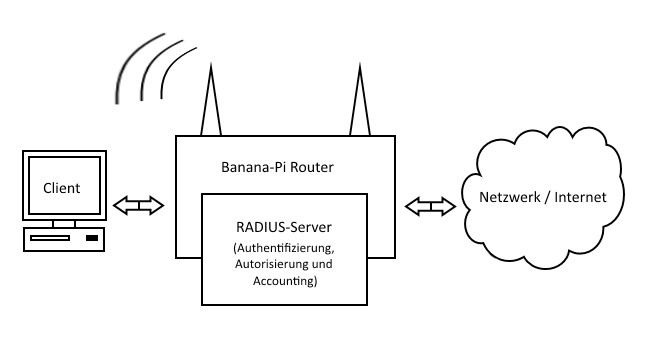
\includegraphics[width=\textwidth]{pictures/Tom/Radius}
\caption{Radius Funktionsweise}
\end{figure}
Anhand der obenstehenden Abbildung lässt sich gut erkennen wie der Aufbau ist. Der Client
(Smartphone, PC, etc.) kann sich wahlweise per WLAN oder LAN mit dem Banana-Pi Router
verbinden, dabei sendet er eine Authentifizierungsanfrage an diesen, welche der Router an den
Radius-Server, welcher auf dem Banana-Pi läuft, weiterleitet. Dieser verarbeitet nun die Anfrage
indem er, je nach Konfiguration, in unserem Fall über eine SQL-Datenbank überprüft ob der Client
berechtigt ist dem Netzwerk beizutreten. Zusätzlich kann diese Verbindung dann auch limitiert
werden (Volumen-Limit, Bandbreiten-Drosselung, beschränkter Zugriff auf Subnetze/VLANs).
\newpage

\subsection{FreeRADIUS}
FreeRADIUS ist wie der Name schon vermuten lässt eine freie und kostenlose Implementierung des
RADIUS-Protokolls und unter der GNU General Public License, version 2 lizenziert. Es ist laut
eigenen Angaben der weltweit am meisten eingesetzte RADIUS-Server und wird von den meisten
Internetdienstanbietern (Providern) sowie den 500 umsatzstärksten Unternehmen der Welt
benutzt. \cite{rad2}\\
Es findet außerdem auch in der Hochschule sowie im akademischen Forschungsnetzwerk Eduroam
Einsatz. Es unterstützt den meistverbreiteten Authentifizierungsstandard EAP, auf deutsch etwa„Erweiterbares Authentifizierungsprotokoll“ \cite{rad3}
, der ca. 40 verschiedene Verfahren anbietet, welche
heutzutage unter anderem in den Sicherheitsimplementationen WPA und WPA2 Verwendung
finden.\\
~\\
Installation:\\
FreeRADIUS ist auch in den offiziellen Paket-Quellen von Debian enthalten und kann somit ganz
einfach über den Debian-Paketmanager apt-get installiert werden. Als erstes stellen wir sicher dass
das System up-to-date ist und die aktuellen Paketquellen besitzt. \cite{rad4}
\begin{lstlisting}
sudo apt-get update
sudo apt-get upgrade
sudo apt-get freeradius freeradius-utils freeradius-mysql mysql-server
\end{lstlisting}
Bei der Installation des MySQL-Servers wird man gebeten das Passwort für den Root-User zu
setzen und zu bestätigen (in unserem Fall ist dies bananapi). Im nächsten Schritt wird eine
Datenbank für RADIUS angelegt.
\begin{lstlisting}
ql -uroot -p
\end{lstlisting}
\begin{lstlisting}
CREATE DATABASE radius;
GRANT ALL PRIVILEGES ON radius.* TO root@localhost IDENTIFIED BY "bananapi";
flush privileges;
exit
\end{lstlisting}
Danach noch die SQL Schemas in die Datenbank laden: \cite{rad5}
\begin{lstlisting}
mysql -uroot -p radius < /etc/freeradius/sql/main/mysql/schema.sql
mysql -uroot -p radius < /etc/freeradius/sql/main/mysql/setup.sql
\end{lstlisting}
Zukünftig können nun Benutzer mit folgendem MySQL-Befehl angelegt werden:
\begin{lstlisting}
insert into radcheck (username,attribute,op,value) values("USERNAME", "Cleartext-Password", ":=", "PASSWORD");
\end{lstlisting}
Nun muss RADIUS dafür konfiguriert werden, das SQL-Modul zu benutzen, dafür editiert man die
Datei /etc/freeradius/sql.conf und trägt im Bereich \#Connection info die korrekten Login-Daten ein.
Desweiteren muss man in der Datei radius.conf die Zeile \$INCLUDE sql.conf, sowie in der Datei
/etc/freeradius/sites-available/default zwei mal sql in den Sektionen authorize { und accounting
{ ein kommentieren.\\
~\\
Testen:\\
Um die Konfiguration zu überprüfen kann der RADIUS-Server im Debugging-Modus gestartet
werden. Dazu sollte der RADIUS-Dienst erst beendet werden:
\begin{lstlisting}
service freeradius stop
freeradius -X
\end{lstlisting}
Danach kann in einem zweiten Terminal (oder ggf. mit Terminal-Multiplexer) das Programm radtest
verwendet werden um Authentifizierungsanfragen an den RADIUS-Server zu senden: \cite{rad6}
\begin{lstlisting}
radtest USERNAME PASSWORD 127.0.0.1 0 mysecret
\end{lstlisting}
Eine typische Ausgabe einer erfolgreichen Anfrage sollte wie folgt aussehen:
\begin{figure}[ht]                    
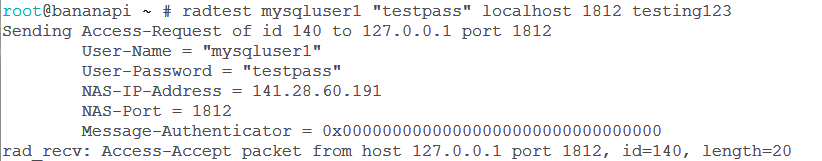
\includegraphics[width=\textwidth]{pictures/Tom/Radius2}
\caption{Radius Test}
\end{figure}
\newpage
\subsection{Inbetriebnahme von FreeRADIUS2 auf OpenWRT}
1. Installation des FreeRADIUS2 mit den üblichen Paketen die von verschiedenen anderen Paketen
benutzt werden:
\begin{lstlisting}
> opkg install freeradius2 freeradius2-common freeradius2-utils
Unknown package 'freeradius2'.
Unknown package 'freeradius2-common'.
Unknown package 'freeradius2-utils'.
Collected errors:
* opkg_install_cmd: Cannot install package freeradius2.
* opkg_install_cmd: Cannot install package freeradius2-common.
* opkg_install_cmd: Cannot install package freeradius2-utils.
\end{lstlisting}
-> Hat nicht funktioniert, auch nach halbstündiger Investigation konnte keine Lösung gefunden
werden, auch mit
\begin{lstlisting}
> opkg search freeradius2
> opkg info freeradius2
\end{lstlisting}
konnten keine Informationen über das Paket ermittelt werden. Schlussendlich konnten die Pakete
über das Web-Interface installiert werden, dort klappte es auf Anhieb (mit den gleichen
Bezeichnern)\\
~\\
2. Installation der FreeRADIUS2 Pakete für die MYSQL Unterstützung (+ Packet für Logging):
\begin{lstlisting}
> opkg install freeradius2-mod-sql freeradius2-mod-sql-mysql freeradius2-mod-sqllog
\end{lstlisting}
Nun sind die benötigten Pakete installiert.\\
\newpage
Die Ausgabe nach der Installation sieht folgendermaßen aus:
\begin{lstlisting}
nstalling freeradius2 (2.2.8-2) to root...
Downloading file:///etc/packages/packages/freeradius2_2.2.8-2_sunxi.ipk.
Installing freeradius2-common (2.2.8-2) to root...
Downloading file:///etc/packages/packages/freeradius2-common_2.2.8-2_sunxi.ipk.
Configuring freeradius2-common.
Configuring freeradius2.
ifconfig: br-lan: error fetching interface information: Device not found
ifconfig: br-lan: error fetching interface information: Device not found
radiusd: Invalid IP Address or hostname "-p"
\end{lstlisting}
Mit br-lan ist hier das sogenannte „bridged lan virtual interface“ gemeint (liegt daran dass es
standardmäßig so vorkonfiguriert ist).\\
Beim Versuch FreeRADIUS2 im Debugging-Modus zu starten kommt:\
\begin{lstlisting}
> radiusd -X
radiusd: FreeRADIUS Version 2.2.8, for host arm-openwrt-linux-gnu, built on Oct 3 2016 at 22:22:30
Copyright (C) 1999-2015 The FreeRADIUS server project and contributors.
There is NO warranty; not even for MERCHANTABILITY or FITNESS FOR A PARTICULAR PURPOSE.
You may redistribute copies of FreeRADIUS under the terms of the GNU General Public License.
For more information about these matters, see the file named COPYRIGHT.
Starting - reading configuration files ...
including configuration file /etc/freeradius2/radiusd.conf
including configuration file /etc/freeradius2/clients.conf
including files in directory /etc/freeradius2/modules/
including configuration file /etc/freeradius2/eap.conf
Unable to open file "/etc/freeradius2/eap.conf": No such file or directory
Errors reading or parsing /etc/freeradius2/radiusd.conf
\end{lstlisting}
EAP ist das Extensible Authentication Protocol, ein allgemeines Authentifizierungsprotokoll. Also
wurden die noch benötigten FreeRADIUS2 Abhängigkeiten Installiert:
\begin{lstlisting}
> opkg install freeradius2-mod-chap freeradius2-mod-detail freeradius2-mod-eap freeradius2-mod-eap-md5 freeradius2-mod-eap-mschapv2 freeradius2-mod-eap-peap freeradius2-mod-eap-tls freeradius2-mod-eap-ttls
freeradius2-mod-exec freeradius2-mod-files freeradius2-mod-logintime
freeradius2-mod-mschap freeradius2-mod-pap freeradius2-mod-passwd
freeradius2-mod-preprocess freeradius2-mod-radutmp
\end{lstlisting}
3. Installation des MYSQL-Servers
\begin{lstlisting}
> opkg install mysql-server
Installing mysql-server (5.1.73-1) to root...
Downloading file:///etc/packages/packages/mysql-server_5.1.73-1_sunxi.ipk.
Installing libmysqlclient (5.1.73-1) to root...
Downloading file:///etc/packages/packages/libmysqlclient_5.1.73-1_sunxi.ipk.
Configuring libmysqlclient.
Configuring mysql-server.
/etc/init.d/mysqld: Error: datadir '/mnt/data/mysql/' in /etc/my.cnf
doesn't exist
\end{lstlisting}
Nach einiger Zeit stieß ich im Internet auf vergleichbare Probleme und es gab einen Work-Around
mit dem der MYSQL-Server sich schließlich doch installieren lies.\\
~\\
4. Einrichtung einer Zertifikatskette für das EAP
\begin{lstlisting}
>opkg install openssl-util
\end{lstlisting}
->Erstellung der Zertifikatskette mit OpenSSL (...)\\
\newpage
5. Bevor man allerdings mit der Konfiguration beginnt, sollte man jedoch den Radius-Daemon
stoppen: Über das Web-Interface LuCi unter dem Menüpunkt „System“ ->„Startup“ wird der
radiusd deaktiviert („disable“) und erstmal vom automatischen Starten beim Booten
ausgenommen. Für Test- und Debuggingzwecke empfiehlt es sich außerdem, den Radius Server
umzukonfigurieren, sodass dieser auch auch auf Localhost horcht und nicht nur auf die IP Adresse
im Netzwerk. Dafür editiert man die Datei
\begin{lstlisting}
> vim /etc/init.d/radiusd
\end{lstlisting}
und ersetzt die Zeile 17
\begin{lstlisting}
radiusd -i $IPADDR -p 1812,1813 $OPTIONS
\end{lstlisting}
durch
\begin{lstlisting}
radiusd $OPTIONS
\end{lstlisting}












